\subsection{Activities}

%%%%%%%%%%%%%%%%%%%%%%%%%%%%%%%%%%%%%%%%%%%%%%%%%%%%%%%%%%%%%%%%%%%%%%

\subsubsection[Hough Transform bibliographical review.]{Hough Transform applications bibliographical review.}
<Pending table>

%%%%%%%%%%%%%%%%%%%%%%%%%%%%%%%%%%%%%%%%%%%%%%%%%%%%%%%%%%%%%%%%%%%%%%

\subsubsection{C implementation of Probabilistic Hough Transform.}

Due to the applications observed in the bibliographical review it was decided that a Probabilistic Hough Transform should be implemented in C. This is, mathematically speaking, not a transform because it can not be reverted.

\begin{figure}[ht!]
\begin{center}
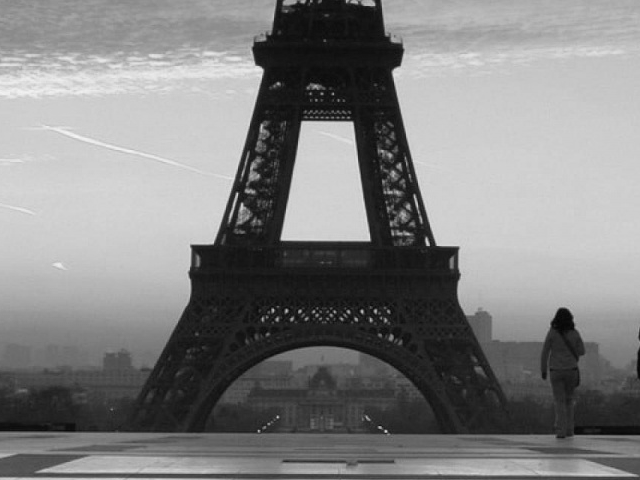
\includegraphics[height=0.4\textwidth]{fig/eiffel_grayscale}\\
\caption{Original Eiffel Tower grayscale image.}
\label{fig_eiffel_grayscale}
\end{center}
\end{figure}

\begin{figure}[ht!]
\begin{center}
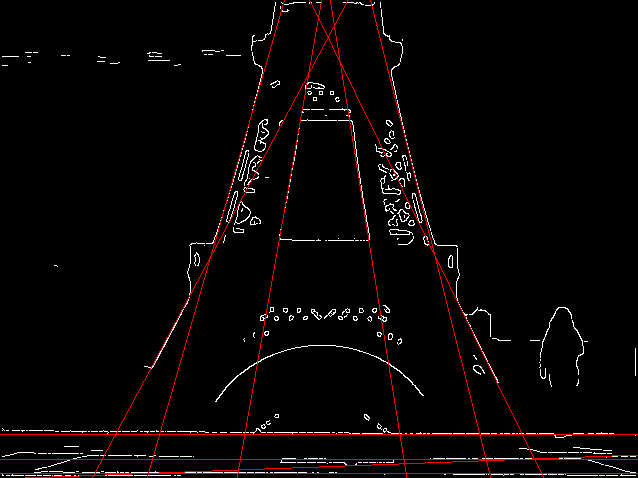
\includegraphics[height=0.4\textwidth]{fig/eiffel_hough}\\
\caption{Eiffel Tower image processed using the Hough Transform.}
\label{fig_eiffel_hough}
\end{center}
\end{figure}

\begin{figure}[ht!]
\begin{center}
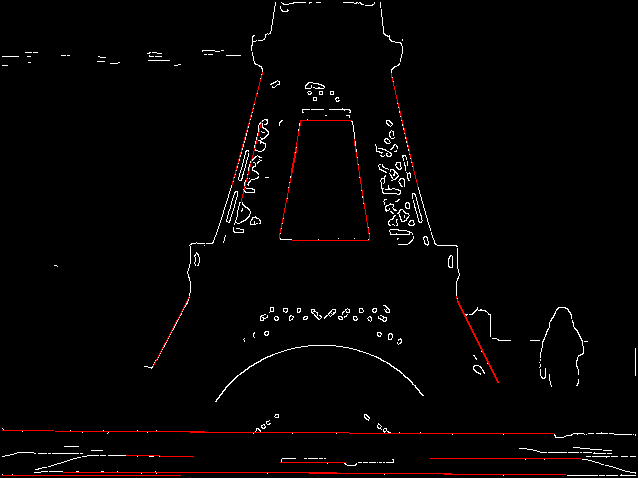
\includegraphics[height=0.4\textwidth]{fig/eiffel_phough}\\
\caption{Eiffel Tower image processed using the Probabilistic Hough Transform.}
\label{fig_eiffel_phough}
\end{center}
\end{figure}


\begin{itemize}
	\item Conceptual variant of the Hough Transform that solves its most important disadvantage.
	\item OpenCV has both implementations: Hough Transform and Probabilistic Hough Transform (most used).
\end{itemize}

\begin{table}
\begin{center}
\begin{tabular}{| l | c | c |}
\hline
\multicolumn{1}{|c|}{Parameter}	 & 	\multicolumn{1}{c|}{Traditional}	 & 	\multicolumn{1}{c|}{Probabilistic}\\ \hline
Total time (s)	& 	163.97	 &	154.52\\ \hline
Time per frame (ms)	& 	20.5	 & 	19.32\\ \hline
Frequency (Hz)		& 	48.79	 & 	51.77\\ \hline
\end{tabular}
\caption[Comparison of Hough transform algorithms.]{Comparison of Hough transform algorithms processing the same image 8000 times.}
\label{tab_compeiffel}
\end{center}
\end{table}


Both implementations were used to process the same image (Fig.~\ref{fig_eiffel_grayscale}) to compare their performance. The graphical result of the traditional algorithm is shown in figure \ref{fig_eiffel_hough}. The output of using the probabilistic variation is shown in figure \ref{fig_eiffel_phough}. Both algorithms were executed eight thousand times on the original images to avoid noise from unrelated software running during the experiment.

The following observations can be from the results:

\begin{itemize}
	\item The traditional algorithm does not compute lines' delimiting points (this is the reason lines cross through all the image).
	\item The probabilistic version detected all (and even more) the lines detected by its counterpart.
	\item A comparison of the time taken by both algorithms is shown in \ref{tab_compeiffel}.
	\item The ammount of time taken by the Probabilistic Hough Transform is slightly lower but it does more than the traditional one. It does much more in slightly less time.
	\item The line extraction parameters of the traditional algorithm are tuned and proved.
	\item Probabilistic Hough Transform parameters can still be tuned to get better results.
\end{itemize}

%%%%%%%%%%%%%%%%%%%%%%%%%%%%%%%%%%%%%%%%%%%%%%%%%%%%%%%%%%%%%%%%%%%%%%

\subsubsection{Planning}
Objectives were classified in the following categories:
\begin{itemize}
	\item \textbf{STM32:} Image acquisition and sending code.
	\item \textbf{Mechanic:} Hardware, mounting the cameras on the vehicle, etcetera.
	\item \textbf{Raspberry:} Image reception code and task management (pririties, scheduler, etcetera).
	\item \textbf{Vision:} Image processing.
	\item \textbf{Control:} Model extraction, control synthesis.
	\item \textbf{Paper:} Researching, documenting and publishing project results.
\end{itemize}
